\section{Reconhecimento dos Usuários}
	 
	O reconhecimento facial do Sistema TRUE foi implementado utilizando imagens de cor como dados de entrada. Portanto, ele tem influência de diversos fatores como iluminação, ângulo, pose, expressões, maquiagem e acessórios. Para análise dos resultados foi utilizada como ferramenta uma matriz de confusão construída a partir dos dados coletados do sistema. Tal matriz contém em suas colunas os valores possíveis que se podem obter para cada usuário e as linhas os usuários que foram observados. Os valores presentes na matriz mostram os resultados, em porcentagens, dos testes de reconhecimento. Cada célula apresenta o percentual de vezes que o resultado (coluna) ocorreu durante os testes com o indivíduo (linha) sendo reconhecido. Desta forma, a matriz permite a fácil visualização da confiança obtida no reconhecimento observando-se os valores obtidos na diagonal principal. Ela representa a conjunção do valor esperado com o indívíduo testado.

	Sumarizando os resultados expressos na matriz apresentamos três taxas calculadas utilizando os três conceitos a seguir:

	\begin{enumerate}
		\item \textbf{Verdadeiro Positivo}: quando o sistema identifica o usuário de maneira correta.
		\item \textbf{Verdadeiro Negativo}: quando o sistema identifica o usuário de maneira errada.
		\item \textbf{Falso Negativo}: quando o sistema não identifica o usuário cadastrado.
	\end{enumerate}

	A taxa de verdadeiro positivo representa a média de acertos do sistema ao identificar os usuários. A taxa de verdadeiro negativo representa a média de erros que houveram ao se reconhecer equivocadamente um usuário como outro. A taxa de falso negativo representa a média de erros que houveram quando um usuário cadastro não foi reconhecido e considerado como ``desconhecido''.

% TODO :voltar aqui

Os cenários de teste utilizados para se averiguar a precisão do reconhecimento
facial consistiram de duas etapas. 
Na primeira etapa cada usuário foi cadastrado
na base de dados utilizando estratégias distintas para cada cenário. A esta
base de dados foram adicionadas os dados das 40 pessoas presentes no banco de faces da Universidade de Cambridge~\cite{cambridgeFaceDb}. Na segunda etapa cada usuário,
individualmente, foi posicionado dentro do campo de visão do sensor onde foram
coletados os resultados dos primeiros 20 valores retornados pelo sistema.
Primeiramente foi construído um cenário de testes que não apresentou resultados
satisfatórios, com isto foi construído um segundo cenário de teste com uma nova
abordagem para a coleta de faces (1ª etapa).

	% Foram realizados dois conjuntos de testes para avaliar a precisão do reconhecimento facial implementado no Sistema TRUE. Os cenários desses testes foram compostos por usuários previamente cadastrados, além das 40 pessoas cadastradas no banco de faces da Universidade de Cambridge~\cite{cambridgeFaceDb}. No primeiro conjunto de testes foram previamente cadastrados 11 usuários e no segundo 10 usuários. Nesses testes, cada usuário se posicionou em frente ao \textit{Kinect}, com o rosto na posição frontal em relação ao sensor. Com isso, o sistema realizou o processo de reconhecimento facial 20 vezes para cada usuário. Os dois conjuntos de testes foram necessários tendo em vista que os resultados do primeiro não foram satisfatórios. A diferença entre ambos está na estratégia utilizada no cadastro dos usuários no sistema. 

		\begin{figure}[htb]
			\begin{center}
				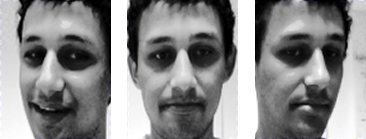
\includegraphics[scale=0.4]{figuras/4.ProblemaEProposta/face-registro.png}
			\end{center}
			\caption{Exemplo de imagens obtidas na etapa de cadastro do usuário.}
			\label{fig:imgs-cadastro}
		\end{figure}	

	No primeiro conjunto de testes, os cadastros dos usuários foram feitos utilizando 10 imagens de faces de cada usuário: 6 imagens frontais da face, 2 imagens da face ligeiramente rotacionada para direita e 2 imagens da face ligeiramente rotacionada para esquerda. A Figura~\ref{fig:imgs-cadastro} exemplifica imagens de face obtidas nestes cadastros. Os cadatros foram realizados com essa estratégia com o objetivo de diminuir o impacto das variações de poses e ângulo no reconhecimento facial. Os resultados obtidos dos processos de reconhecimento facial realizados para cada usuário são mostrados na matriz de confusão representada pela Tabela~\ref{tab:matriz-confusao}. 

	\begin{table}[htb]
		\begin{center}
			\caption{Matriz de confusão para apresentar os resultados obtidos no primeiro conjunto de testes.}
			\label{tab:matriz-confusao}
			\begin{tabular}{|c|c|c|c|c|c|c|c|c|c|c|c|c|}
				\hline  & \bf \begin{sideways}Tales\end{sideways} & \bf \begin{sideways}Danilo\end{sideways} & \bf \begin{sideways}Ana\end{sideways} & \bf \begin{sideways}Fabricio\end{sideways} & \bf \begin{sideways}Lucas\end{sideways} & \bf \begin{sideways}Bruno\end{sideways} & \bf \begin{sideways}Ricardo\end{sideways} & \bf \begin{sideways}Estevao\end{sideways} & \bf \begin{sideways}Rafael\end{sideways} &
				\bf \begin{sideways}Vinicius\end{sideways} & \bf \begin{sideways}Pedro\end{sideways} & \bf \begin{sideways}Desconhecido\end{sideways}\\ 
				
				\hline \bf Tales 		& 95\% & 			& 		 & 			&   	 & 			& 		 & 			& 		 & 			& 		 & 5\%	\\ 
				\hline \bf Danilo 	& 		 & 75\% & 		 & 			&   	 & 			& 		 & 			& 		 & 			& 25\% &		 	\\
				\hline \bf Ana 			& 		 & 			& 95\% & 			&   	 & 			& 		 & 			& 		 & 			& 		 & 5\%  \\
				\hline \bf Fabricio & 20\% & 			& 		 & 50\% &      & 			& 10\% & 			&  	   & 20\% & 		 &		  \\
				\hline \bf Lucas 		& 		 & 			& 		 & 			& 55\% & 			& 		 & 			& 		 & 			& 20\% & 25\% \\
				\hline \bf Bruno 		& 5\%	 & 			& 		 & 			& 		 & 70\% & 		 & 			& 10\% & 	5\%	& 		 & 10\%	\\
				\hline \bf Ricardo 	& 		 & 			& 10\% & 			& 		 & 			& 85\% & 			& 		 & 			& 		 & 5\%  \\
				\hline \bf Estevao 	& 		 & 			& 		 & 			& 		 & 			& 		 & 70\% & 		 & 			& 		 & 30\% \\
				\hline \bf Rafael 	& 10\% & 	5\%	& 		 & 			& 10\% & 			& 		 & 			& 45\% & 20\% & 		 & 10\% \\
				\hline \bf Vinicius & 		 & 			& 5\%  & 			& 		 & 			& 		 & 			& 5\%  & 70\% & 10\% & 10\% \\
				\hline \bf Pedro 		& 		 & 			& 		 & 			& 		 & 			& 		 & 			& 		 & 			& 100\%&		  \\
				\hline
			\end{tabular}
		\end{center}
	\end{table}

	Como previsto, pode-se observar na matriz que os valores mais significativos estão na diagonal principal. Alguns resultados obtidos foram satisfatórios com porcentagens maiores que 90\%. Por outro lado, foram obtidos alguns resultados com baixas porcentagens como 45\%. Estes últimos foram principalmente causados por problemas como pose e expressões faciais. A iluminação não foi um problema, pois no ambiente de teste não existe influência da iluminação externa e a interna é controlada. 

	A Tabela~\ref{tab:taxas} apresenta as taxas de Verdadeiro Positivo, Verdadeiro Negativo e Falso Negativo calculadas analisando os valores da Tabela~\ref{tab:matriz-confusao}. Observa-se que a taxa de verdadeiro positivo (73,63\%) foi uma taxa baixa para um sistema de reconhecimento automático. Neste conjunto de testes, a taxa de verdadeiro negativo foi bem superior a taxa de falso negativo mostrando que a principal deficiência do reconhecimento facial consiste na confusão entre os usuários cadastrados no sistema.


	Como dito anteriormente, os resultados deste primeiro cenário não se mostrou satisfatório. Sob a hipótese do resultado ter sido influencidado pela baixa quantidade de faces e poses, construiu-se um segundo cenário de testes. Neste a estratégia utilizada nos cadastros do usuários foi diferente. Os cadastros foram feitos utilizando 100 imagens das faces de cada usuário em diferentes ângulos, posições e expressões faciais. No momento do cadastro, foi solicitado que os usuários movimentasse o rosto levementa para cima, para baixo, para esquerda e para direira de maneira aleatória e com diferentes expressões faciais. Os resultados obtidos neste conjunto de testes se econtra na segunda matriz de confusão mostrada na Tabela~\ref{tab:matriz-confusao2}.

	\begin{table}[htb]
		\begin{center}
			\caption{Taxas obtidas para o primeiro conjunto de testes de identificação.}
			\label{tab:taxas}
			\begin{tabular}{|l|c|}
				\hline \bf Verdadeiro Positivo & 73,63\% \\
				\hline \bf Verdadeiro Negativo & 17,27\% \\
				\hline \bf Falso Negativo & 9,10\% \\
				\hline
			\end{tabular}
		\end{center}
	\end{table}


	% \begin{table}[htb]
	% 	\begin{center}
	% 		\caption{Matriz de confusão para apresentar os resultados obtidos.}
	% 		\label{tab:matriz-confusao2}
	% 		  \begin{tabular}{|c|c|c|c|c|c|c|c|c|}
	% 			% \hline  & \bf \ref{user:tales} & \bf \ref{user:danilo} & \bf
	% 			% \ref{user:ana} & \bf \ref{user:fabricio} & \bf \ref{user:lucas} & \bf
	% 			% \ref{user:bruno} &  \bf Desconhecido\\

	% 			\hline  & \bf Tales & \bf Danilo & \bf Ana & \bf Fabricio & \bf Lucas & \bf Bruno &  \bf Desconhecido\\
				 
	% 			\hline \bf Tales 		& 90\% & 			& 		 & 			&   	 & 			& 10\%		\\
	% 			\hline \bf Danilo 	& 		 & 100\%& 		 & 			&   	 & 			& 		 		\\
	% 			\hline \bf Ana 			& 		 & 			& 100\%& 			&   	 & 			& 		    \\
	% 			\hline \bf Fabricio & 		 & 			& 		 &100\%      &      & 			&      		\\
	% 			\hline \bf Lucas 		& 		 & 			& 		 & 			& 85\% & 			& 15\%		\\
	% 			\hline \bf Bruno 		& 		 & 			& 		 & 			& 		 & 100\%& 		  	\\
	% 			\hline
	% 		\end{tabular}
	% 	\end{center}
	% \end{table}

	\begin{table}[htb]
		\begin{center}
			\caption{Matriz de confusão para apresentar os resultados obtidos no segundo conjunto de testes.}
			\label{tab:matriz-confusao2}
			  \begin{tabular}{|c|c|c|c|c|c|c|c|c|c|c|c|c|}
				% \hline  & \bf \ref{user:tales} & \bf \ref{user:danilo} & \bf
				% \ref{user:ana} & \bf \ref{user:fabricio} & \bf \ref{user:lucas} & \bf
				% \ref{user:bruno} &  \bf Desconhecido\\

				\hline  & \bf \begin{sideways}Tales\end{sideways} & \bf \begin{sideways}Danilo\end{sideways} & \bf \begin{sideways}Ana\end{sideways} & \bf \begin{sideways}Fabricio\end{sideways} & \bf \begin{sideways}Lucas\end{sideways} & \bf \begin{sideways}Bruno\end{sideways} & \bf \begin{sideways}Carla\end{sideways} & \bf \begin{sideways}Marcela\end{sideways} & \bf \begin{sideways}Caio\end{sideways} & \bf \begin{sideways}Marcelo\end{sideways} & \bf \begin{sideways}Desconhecido\end{sideways}\\
				 
				\hline \bf Tales 			&100\% & 			& 		 & 			&   	 & 			& 		& 		&	 		& 		& 		\\
				\hline \bf Danilo 		& 		 &100\%	& 		 & 			&   	 & 			& 		& 		& 		& 		& 		 		\\
				\hline \bf Ana 				& 		 & 			& 100\%& 			&   	 & 			& 		& 		& 		& 		& 		    \\
				\hline \bf Fabricio 	& 		 & 			& 		 &45\%	&      & 			& 		& 		& 		& 5\%	& 50\%    		\\
				\hline \bf Lucas 			& 		 & 			& 		 & 			& 85\% & 			& 		& 		& 		& 		& 15\%		\\
				\hline \bf Bruno 			& 		 & 			& 		 & 			& 		 & 75\% & 	  & 		&20\% & 5\%	& 		  	\\
				\hline \bf Carla 			& 		 & 			& 		 & 			& 		 & 			&85\% &		  & 	  & 		& 15\%		  	\\
				\hline \bf Marcela 		& 		 & 			& 		 & 			& 		 &      & 		&65\% &10\% & 		& 25\%		  	\\
				\hline \bf Caio 		  & 		 & 			& 		 & 			& 	5\%& 	15\%& 		& 		&80\%	&	 		& 		  	\\
				\hline \bf Marcelo 		& 		 & 			& 		 & 			& 		 & 			& 		& 		& 		& 90\%& 10\%		  	\\
				\hline
			\end{tabular}
		\end{center}
	\end{table}

	\begin{table}[htb]
		\begin{center}
			\caption{Taxas obtidas para o segundo conjunto de testes de identificação.}
			\label{tab:taxas2}
			\begin{tabular}{|l|c|}
				\hline \bf Verdadeiro Positivo & 82,5\% \\
				\hline \bf Verdadeiro Negativo & 6,0\% \\
				\hline \bf Falso Negativo & 11,5\% \\
				\hline
			\end{tabular}
		\end{center}
	\end{table}

	% "Ao analisar os dados da Tabela 5.5 pode-se observar que os resultados melhoraram significamente." => "Observa-se uma melhora siginifcativa nos resultados expressos na Tabela 5.6 com relação aos apresentados na Tabela 5.5."

	Observa-se uma melhora siginifcativa nos resultados expressos na Tabela~\ref{tab:matriz-confusao2} com relação aos apresentados na Tabela~\ref{tab:matriz-confusao}. A Tabela~\ref{tab:taxas2} apresenta as taxas de acerto e erros relativos à Tabela~\ref{tab:matriz-confusao2}. Houve um aumento na taxa de Verdadeiro Positivo de 73,63\% para 82,5\% e redução significativa na taxa de Verdadeiro Negativo de 17,27\% para 6,0\%, mostrando que os casos de confusões entre os usuários foram mais raros. A melhora obtida comprova a hipótese que um número maior de poses e faces aprimorou a capacidade do sistema de reconhecer seus usuários. Este acréscimo de informações torna os resultados mais robustos devido a inclusão de informações de mais cenários dos usuários no sistema. 

	% Para esta matriz obtemos as taxas apresentadas na Tabela~\ref{tab:taxas2}. É
	% possível observar que o método de cadastro influi bastante no resultado final.
	% Também é possível inferir que quanto maior a variância das imagens para um
	% mesmo usuário melhor o seu reconhecimento.

